\chapter{Các kết quả thí nghiệm}
\label{Chapter4}

\textit{Trong chương này, chúng tôi tiến hành các thí nghiệm nhằm kiểm chứng lý thuyết về thuật toán Adam đã trình bày ở chương 3. Trước hết, để so sánh kết quả cài đặt của chúng tôi với kết quả được công bố trong bài báo gốc, chúng tôi thí nghiệm huấn luyên mạng “Multi-layer Neural Network” trên bộ dữ liệu ảnh nhỏ là MNIST và mạng "Convolutional Neural Network" trên bộ dữ liệu ảnh trung là CIFAR10. Tiếp theo, chúng tôi thực hiện thí nghiệm trực quan hóa cách Adam và các thuật toán khác di chuyển trong trường hợp bề mặt lỗi có dạng rãnh hẹp và rãnh rất hẹp; dữ liệu được sử dụng trong thí nghiệm này là dữ liệu tự tạo và ít chiều để có thể trực quan hóa. Cuối cùng, để thấy rõ hơn về hiệu quả của Adam so với các thuật toán khác trong ngữ cảnh thực tế, chúng tôi thí nghiệm huấn luyện mạng "Convolutional Neural Network" trên bộ dữ liệu ảnh lớn là ImageNet và mạng "Long Short-term Memory" trên bộ ngữ liệu là Penn Treebank.}

\section{Các thiết lập thí nghiệm}

Chúng tôi thực hiện hai loại thí nghiệm: thí nghiệm nguyên lý và thí nghiệm thực tế. Trong các thí nghiệm nguyên lý, chúng tôi sử dụng hàm số để tạo ra dạng địa hình bề mặt lỗi mong muốn. Ngoài ra, chúng tôi cũng tạo một bộ dữ liệu ngẫu nhiên cho các thí nghiệm sử dụng minibatch. Với các thí nghiệm thực tế, chúng tôi sử dụng nhiều bộ dữ liệu khác nhau cùng với các kiến trúc mạng nơ-ron nhiều tầng ẩn được sử dụng để giải quyết các bài toán ứng dụng hiện nay. Những bộ dữ liệu thực tế mà chúng tôi sử dụng:

\begin{itemize}
	\item MNIST \cite{lecun2010mnist}: Bộ dữ liệu này gồm các ảnh xám của các chữ số viết tay từ 0 đến 9 có kích thước 28x28. Tập dữ liệu gồm 60000 ảnh huấn luyện và 10000 ảnh kiểm tra.
	\item CIFAR10 \cite{krizhevsky2009cifar10}: Bộ dữ liệu này gồm các ảnh màu của 10 lớp đối tượng có kích thước 32x32. Tập dữ liệu có tổng cộng 60000 ảnh, mỗi lớp đối tượng có 6000 ảnh. Trong đó 50000 ảnh được chọn làm ảnh huấn luyện và 10000 ảnh kiểm tra. Bộ dữ liệu này và MNIST là những bộ dữ liệu cơ bản phổ biến để huấn luyện các thuật toán học máy và mạng nơ-ron nhiều tẩng ẩn đơn giản.
	\item ImageNet \cite{deng2009imagenet}: Đây là một trong những bộ dữ liệu hình ảnh lớn nhất hiện nay, thường được dùng để kiểm tra khả năng của các phương pháp thị giác máy tính mới nhất. Phiên bản của bộ dữ liệu mà chúng tôi sử dụng là phiên bản được sử dụng trong thử thách ImageNet Large Scale Visual Recogition Challenge 2012 (ILSVRC2012), với hơn 1.2 triệu ảnh được gán nhãn vào 1000 lớp đối tượng được sử dụng để huấn luyện, và 50000 ảnh để kiểm thử.
	\item Penn Treebank \cite{marcus1993ptb}: Đây là bộ dữ liệu do Marcus và cộng sự tổng hợp gồm 929 000 từ dùng để huấn luyện, 73 000 từ cho tập kiểm thử và 82 000 từ để kiểm tra. Tập dữ liệu gồm có 10 000 từ trong tập từ điển. Tập dữ liệu đã được qua xử lý được lấy từ trang web của Tomas Mikolov (\url{http://www.fit.vutbr.cz/~imikolov/rnnlm/simple-examples.tgz}).
\end{itemize}

Chúng tôi sử dụng ngôn ngữ lập trình Python và thư viện Numpy cho các thí nghiệm nguyên lý, thư viện Pytorch cho các thí nghiệm thực tế. Cả thư viện Numpy và Pytorch đều cung cấp khả năng tăng tốc thực thi bằng việc véc-tơ hóa tính toán trên nền C/C++. Thư viện Numpy tập trung vào các chức năng tính toán đại số trên CPU, phù hợp với các thí nghiệm đơn giản; trong khi thư viện Pytorch là một thư viện máy học có thể xây dựng các mạng nơ-ron nhiều tầng ẩn phức tạp cùng với khả năng thực thi song song trên GPU. Loại GPU mà chúng tôi sử dụng là NVIDIA RTX 2080, ngoài ra chúng tôi cũng sử dụng NVIDIA Tesla T4 và TPU (Tensor Processing Unit) trên nền tảng Google Cloud.

Trong tất cả các thí nghiệm, tất cả các thuật toán tối ưu đều có chung điểm xuất phát: bộ trọng số ban đầu đầu của mạng nơ-ron nhiều tầng ẩn sau khi khởi tạo ngẫu nhiên lần đầu sẽ được lưu lại; và với mỗi thuật toán tối ưu được thử nghiệm, bộ trọng số này sẽ được nạp lại vào mạng nơ-ron rồi từ đó mới bắt đầu tiến hành tối ưu và ghi nhận lại kết quả. Điều này giúp đảm bảo sự công bằng cho tất cả các thuật toán khi tiến hành thử nghiệm, tránh được trường hợp một thuật toán nào đó "may mắn" được bắt đầu ở một điểm thuận lợi hơn và nhờ vậy mà hội tụ nhanh hơn.

\begin{center}
	\begin{table}
		\begin{tabularx}{\textwidth}{{|l|l|X|X|}}
			\hline
			\textbf{Thuật toán} & \textbf{Tỉ lệ học} & \textbf{Momentum/$\beta_1$} & \textbf{Alpha/$\beta_2$} \\
			\hline
			SGD & [0.0001, 1] & - & - \\
			\hline
			Momentum & [0.0001, 0.1] & [0.1, 0.99] & - \\
			\hline
			Adagrad & [0.0001, 0.1] & - & - \\
			\hline
			RMSprop & [0.0001, 0.1] & - & [0.9, 0.999] \\
			\hline
			Adam & [0.0001, 0.1] & [0.1, 0.99] & [0.9, 0.999] \\
			\hline
		\end{tabularx}
	\caption{\label{tab:hparam-search}Khoảng giá trị để dò tìm siêu tham số tốt nhất của các thuật toán tối ưu.}
	\end{table}
\end{center}

\section{Các kết quả thí nghiệm}

\subsection{Kết quả của thuật toán cài đặt so với bài báo}
\label{exp:replicate}

Trong phần này, chúng tôi trình bày kết quả của các thuật toán tối ưu mà chúng tôi cài đặt. Cụ thể, chúng tôi so sánh kết quả của các thuật toán do chúng tôi cài đặt lại trên nền thư viện Pytorch với kết quả được công bố trong bài báo thí nghiệm ``Multi-layer Neural Network'' trên tập dữ liệu MNIST và thí nghiệm ``Convolutional Neural Network'' trên tập dữ liệu CIFAR10. Việc tái tạo các kết quả được công bố gặp nhiều khó khăn do bản chất ngẫu nhiên của SGD và dropout, cộng với việc tác giả không công bố các siêu tham số cho các thí nghiệm cũng như các cài đặt liên quan khác. Bài báo cũng không đề cập các khoảng tìm kiếm cho quá trình tìm siêu tham số tối ưu nhất của mỗi thuật toán, vì vậy chúng tôi đã tham khảo các công trình nghiên cứu khác sử dụng các tối ưu này, và tổng hợp các giá trị nhỏ nhất và lớn nhất cho từng siêu tham số của mỗi thuật toán để làm khoảng tìm kiếm (bảng \ref{tab:hparam-search}). Bài báo thực hiện thí nghiệm với thuật toán Nesterov \cite{nesterov1983amf}, Adagrad, RMSprop, AdaDelta \cite{zeiler2012adadelta} và Adam; tuy nhiên chúng tôi nhận thấy rằng Nesterov và AdaDelta không liên quan trực tiếp đến thuật toán Adam mà khóa luận tập trung tìm hiểu, vì vậy chúng tôi sẽ tập trung thực hiện thí nghiệm trên các thuật toán SGD, Momentum, Adagrad, RMSprop, và Adam.

Trong thí nghiệm Multi-layer Neural Network, kết quả mà chúng tôi cài đặt so với kết quả được công bố trong bài báo xấp xỉ nhau về đường đi và vị trí tương đối giữa các thuật toán với nhau (hình \ref{fig:exp-mlp}). Tuy nhiên, giá trị độ lỗi trong cài đặt của chúng tôi cũng thấp hơn đáng kể so với kết quả trong bài báo.

\begin{figure}[htp]
	\centering
	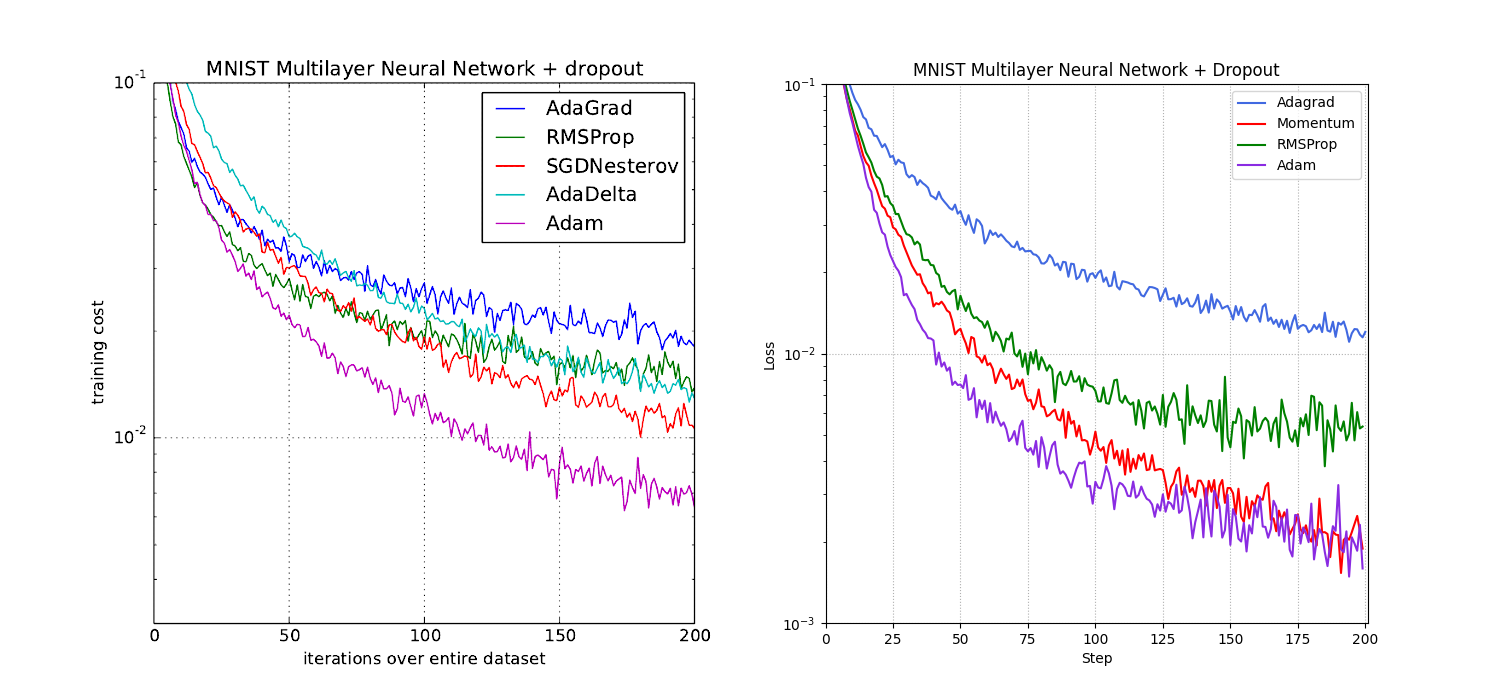
\includegraphics[width=160 mm]{images/mlp.png}
	\caption{Kết quả thí nghiệm Multi-layer Neural Network giữa thuật toán mà chúng tôi cài đặt so với bài báo. Bên trái: kết quả mà bài báo công bố. Bên phải: kết quả do chúng tôi tự cài đặt lại.}
	\label{fig:exp-mlp}
\end{figure}

Nhìn chung, thuật toán Adam có tốc độ tối ưu độ lỗi nhanh nhất trong tất cả các thuật toán được thử nghiệm. Điểm yếu của Adagrad về tỉ lệ học luôn giảm dần được thể hiện rõ khi Adagrad chuyển hướng đi ngang dần mặc dù độ lỗi vẫn cao trong khi các thuật toán khác tiếp tục đi xuống. Điều đó cho thấy rằng mô hình vẫn đang trong quá trình học dữ liệu, nhưng vì tỉ lệ học quá nhỏ nên ở mỗi bước, lượng cập nhật trọng số không đủ để cải thiện mô hình. Vấn đề tỉ lệ học giảm dần do cộng dồn gradient bình phương của Adagrad được RMSprop khắc phục bằng một tỉ lệ suy biến, giúp RMSprop bắt kịp gần hơn với Momentum và Adam. Sự chênh lệch lớn nhất giữa các kết quả nằm ở 2 thuật toán Momentum và Nesterov. Mặc dù 2 thuật toán này chỉ có một sự khác nhau nhỏ ở cách mà quán tính được sử dụng, với Nesterov là phiên bản cố gắng cải thiện hướng cập nhật cho Momentum, tuy nhiên kết quả lại cho thấy Momentum có kết quả tốt hơn khi đạt được độ lỗi thấp hơn RMSprop và ngang bằng với Adam ở các bước cuối cùng.

Trong thí nghiệm Convolutional Neural Network, chúng tôi cũng thực hiện tìm bộ siêu tham số đem lại kết quả cuối cùng thấp nhất cho mỗi thuật toán. Tuy nhiên, sau khi đã tìm được những bộ siêu tham số cho tất cả các thuật toán và thực hiện thí nghiệm, chúng tôi thấy được rằng hầu hết các thuật toán trong cài đặt của chúng tôi đều giúp mô hình đạt được độ lỗi thấp hơn đáng kể so với bài báo khi không dùng dropout. Các giá trị siêu tham số được sử dụng được trình bày chi tiết trong bảng \ref{tab:cnn-hparam}.

Từ hình \ref{fig:exp-cnn-best}, chúng ta có thể thấy rằng bề mặt lỗi của thí nghiệm này có một đoạn dốc xuống khá rõ rệt, và các thuật toán SGD, Momentum cũng như Adam đều giảm độ lỗi rất nhanh khi tìm thấy đoạn dốc ấy. Trong bài báo gốc, một số thuật toán tìm thấy đoạn dốc này ngay từ những epoch đầu tiên, trong khi cài đặt của chúng tôi chỉ bắt đầu giảm mạnh từ khoảng epoch thứ 15. Trong kết quả của chúng tôi, SGD là thuật toán đầu tiên tìm ra đoạn dốc, nhưng độ lỗi tại epoch cuối lại hơi cao hơn so với Momentum và Adam. Có thể là do SGD bị giới hạn bởi tỉ lệ học trong khi hai thuật toán kia có cơ chế tăng tốc giúp đạt được độ lỗi thấp. Kết quả độ lỗi và thời gian thực thi được trình bày trong bảng \ref{tab:cnn-results}.

\begin{figure}[H]
	\centering
	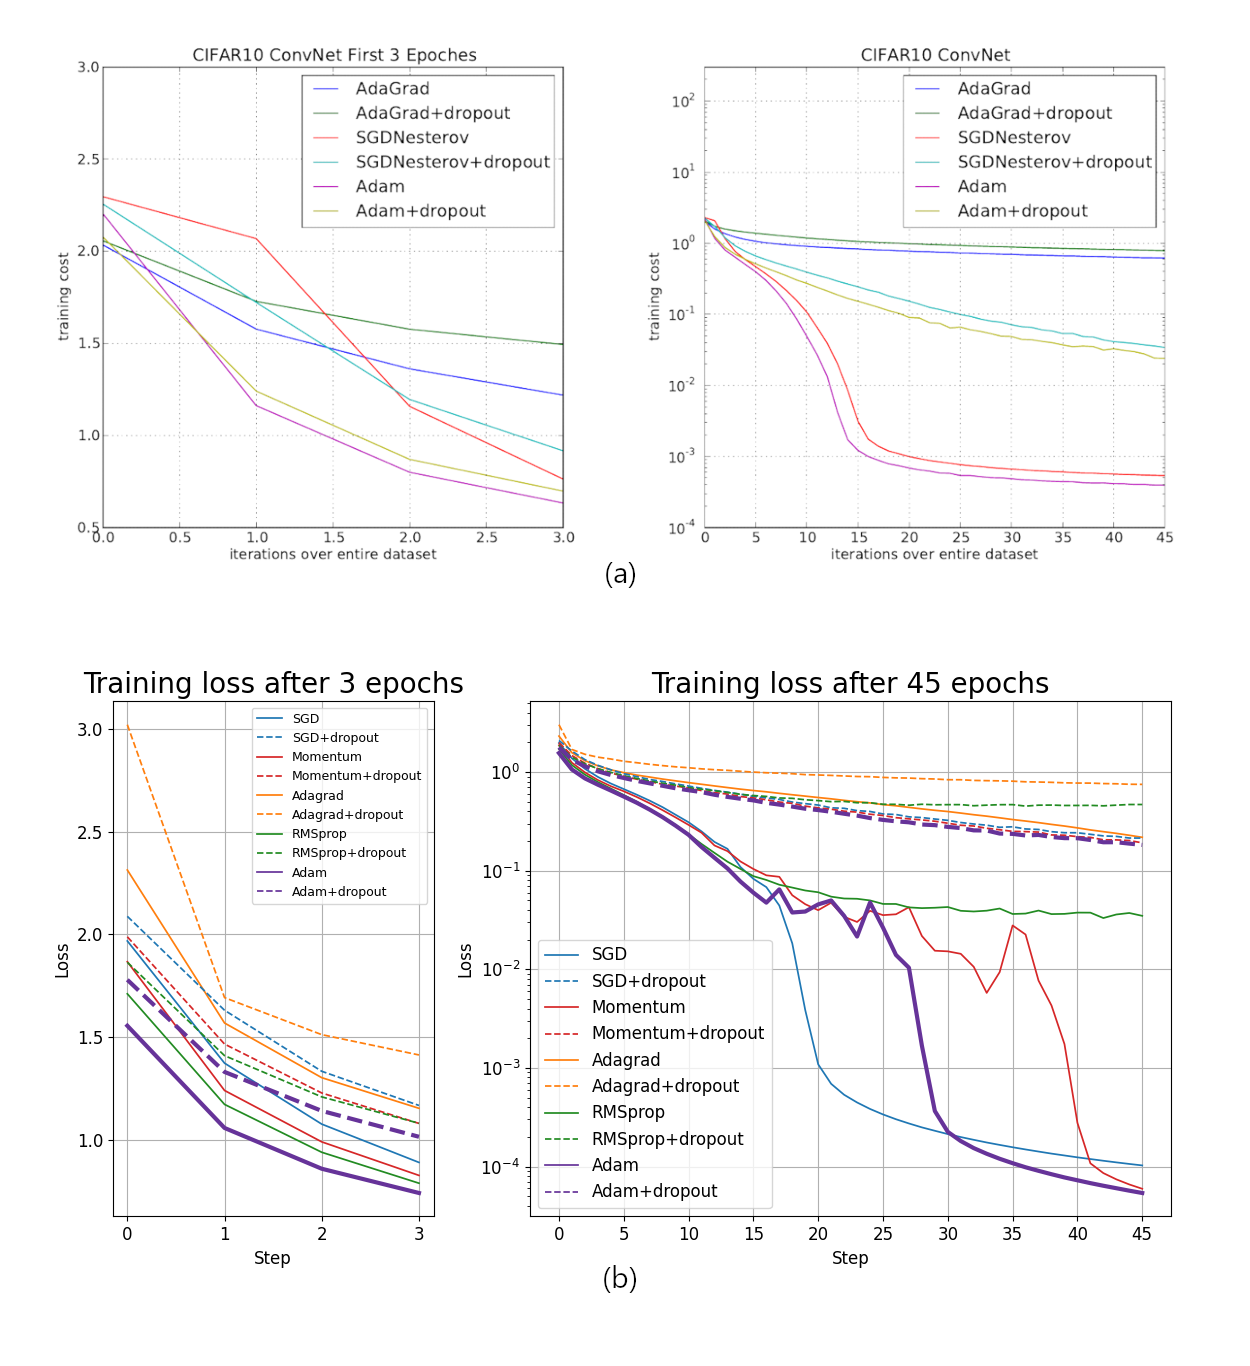
\includegraphics[width=140 mm]{images/cnn.png}
	\caption{Kết quả thí nghiệm Convolutional Neural Network giữa thuật toán mà chúng tôi cài đặt so với bài báo. (a): kết quả mà bài báo công bố. (b): kết quả do chúng tôi tự cài đặt lại.}
	\label{fig:exp-cnn-best}
\end{figure}

\begin{table}
	\begin{tabular}{|m{0.3\textwidth}|>{\raggedright\arraybackslash}m{0.33\textwidth}|m{0.3\textwidth}|}
		\hline
		\textbf{Thuật toán} & \textbf{Thời gian thực hiện (giây)} & \textbf{Độ lỗi thấp~nhất} \\
		\hline
		SGD              & \textbf{6.02 $\pm$ 0.07} & 0.0001 \\
		SGD+dropout      & \textbf{6.04 $\pm$ 0.07} & 0.2139 \\
		\hline
		Momentum         & 6.10 $\pm$ 0.07          & 0.00006 \\
		Momentum+dropout & 6.08 $\pm$ 0.07          & 0.1914 \\
		\hline
		Adagrad          & 6.14 $\pm$ 0.09          & 0.2178 \\
		Adagrad+dropout  & 6.16 $\pm$ 0.09          & 0.7496 \\
		\hline
		RMSprop          & 6.16 $\pm$ 0.07          & 0.03307 \\
		RMSprop+dropout  & 6.19 $\pm$ 0.07          & 0.4512 \\
		\hline
		Adam             & 6.19 $\pm$ 0.07          & \textbf{0.000054} \\
		Adam+dropout     & 6.23 $\pm$ 0.07          & \textbf{0.1824} \\
		\hline
	\end{tabular}
\caption{\label{tab:cnn-results}Kết quả và thời gian thực hiện một epoch của các thuật toán trong thí nghiệm Convolutional Neural Network.}
\end{table}

Về mặt thời gian tính toán, bảng \ref{tab:cnn-results} cho thấy với cùng một kích thước minibatch, có thể dễ hiểu khi SGD cho thời gian tính toán nhanh nhất vì thuật toán này chỉ tính gradient và cập nhật trọng số. Với Momentum, bước tính véc-tơ quán tính $v_t$ trước khi cập nhật trọng số làm tăng thời gian thực hiện mỗi epoch thêm khoảng 15$\%$. Bước tính đường chéo ma trận $G_t$ của các thuật toán tỉ lệ học thích ứng tốn nhiều thời gian hơn đáng kể, vì trong bước này còn có thao tác bình phương các phần tử trong véc-tơ gradient trước khi cộng dồn (thuật toán RMSprop có thêm bước nhân các phần tử này với hệ số suy biến). Adam kết hợp các bước tính quán tính trong Momentum và thích ứng tỉ lệ học, vì vậy Adam có thời gian thực thi chậm nhất trong tất cả các thuật toán.

Ngoài việc tìm bộ siêu tham số cho kết quả tốt nhất, chúng tôi cũng cố gắng tái tạo kết quả mà bài báo đã công bố. Chúng tôi thực hiện quá trình tái tạo này để kiểm tra tính khả thi của các kết quả mà bài báo đã công bố (phụ lục \ref{Appendix2}). Nhìn chung, chúng tôi có thể tái tạo các kết quả thí nghiệm mà bài báo công bố. Tuy nhiên, các kết quả tốt nhất của chúng tôi có độ lỗi thấp hơn đáng kể so với bài báo, đặc biệt là trong thí nghiệm Convolutional Neural Network. Vì không biết chính xác quá trình cài đặt và các siêu tham số đã được sử dụng trong bài báo gốc nên chúng tôi không thể khẳng định nguyên nhân của sự chênh lệch này.

\subsection{So sánh Adam với các thuật toán khác trong trường hợp bề mặt lỗi có dạng rãnh hẹp}

\subsubsection{Rãnh hẹp với các hướng có độ cong khác nhau trùng với trục trọng số}
\label{exp:step-size}

Trong thí nghiệm này, chúng tôi kiểm chứng các khó khăn của dạng địa hình rãnh hẹp và cách các thuật toán khác nhau di chuyển trong đó. Vùng rãnh hẹp là vùng mà độ cong giữa các chiều có sự chênh lệch rất lớn. Cụ thể hơn, một số hướng sẽ có độ cong rất lớn trong khi các hướng khác lại rất bằng phẳng. Vì vậy, để có thể di chuyển hiệu quả trong địa hình này, chúng ta cần giảm kích thước bước cập nhật trên các chiều có độ cong lớn để tránh hiện tượng dao động, đồng thời cập nhật những bước dài hơn trên các chiều bằng phẳng có giá trị gradient nhỏ.

Chúng tôi sử dụng một hàm lỗi giả lập có 2 tham số với sự chênh lệch độ cong trên mỗi trục là rất lớn để tạo thành rãnh hẹp. Gradient của hàm mục tiêu tại vị trí đang xét mà các thuật toán sử dụng có thể được coi như gradient của cả tập dữ liệu. Tất cả các thuật toán đều có cùng một điểm xuất phát.

\begin{figure}[htp]
	\centering
	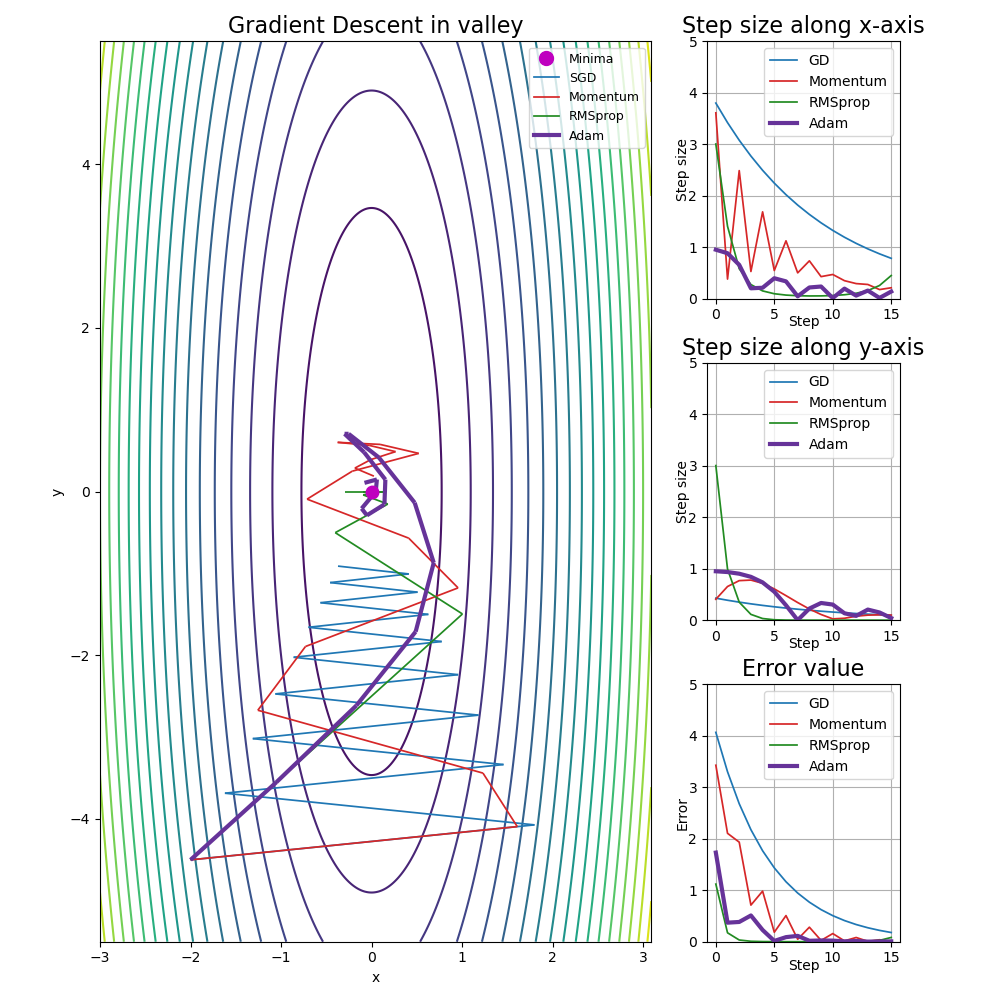
\includegraphics[width=140 mm]{images/step-size.png}
	\caption{Đường đi, độ lớn bước cập nhật theo từng chiều, và độ lỗi của các thuật toán trong quá trình tối ưu hàm giả lập.}
	\label{fig:aligned-step-size}
\end{figure}

Phân tích kết quả chạy thí nghiệm ở hình \ref{fig:aligned-step-size}, ta thấy Adam là thuật toán tối ưu độ lớn bước cập nhật trên cả trục $x$ và trục $y$ tốt nhất. Ta thấy rằng, trong khi các thuật toán khác có độ lớn bước cập nhật đầu khá lớn (RMSProp là 3 ở cả hai trục) hoặc rất khác nhau (Momentum có độ lớn trên trục $x$ lớn hơn trên trục $y$ gấp gần 4 lần), Adam giữ độ lớn của bước cập nhật đầu tiên khá gần nhau và ở giá trị nhỏ (độ lớn bước cập nhật trên cả hai trục là xấp xỉ nhau và gần bằng 1).

Adam giúp giảm dao động tốt hơn Momentum. Trên trục có độ dốc cao $x$, mặc dù độ lớn bước cập nhật của Adam và Momentum đều giảm dần khi tiến càng gần về cực tiểu nhưng Adam cho biên độ dao động nhỏ hơn Momentum rất nhiều thể hiện Adam hạn chế dao động tốt hơn Momentum. Ngược lại trên trục có độ dốc thấp $y$, Adam tăng cường bước cập nhật hiệu quả hơn Momentum khi biên độ dao động độ lớn bước cập nhật của Adam lớn hơn Momentum.

Sự dao động trên cả hai trục cũng giúp cho Adam hoạt động tốt hơn RMSprop với độ lớn bước cập nhật giảm dần ở cả hai trục. Ngoài ra, Adam còn khắc phục nhược điểm gây ra do xấp xỉ bậc hai ở vùng gần cực tiểu tốt hơn RMSprop. Điều này được thể hiện ở các bước cập nhật cuối trên trục có độ dốc cao, RMSprop cho bước cập nhật cuối lớn hơn đáng kể các thuật toán như Adam và Momentum. Đó là lý do vì sao Adam có độ lỗi thấp hơn RMSprop mặc dù đường đi của Adam đi lố qua cực tiểu nhiều hơn RMSprop.

\subsubsection{Rãnh hẹp với các hướng có độ cong khác nhau không trùng với các trục trọng số}
\label{exp:aligned-nonaligned}

Từ nội dung đã trình bày ở chương \ref{Chapter3}, các thuật toán tỉ lệ học thích ứng thay đổi tỉ lệ học theo từng trọng số riêng biệt. Vì vậy, dạng địa hình rãnh hẹp có các hướng trùng với trục của trọng số sẽ là trường hợp mà các thuật toán tỉ lệ học thích ứng phát huy hiệu quả cao nhất. Ngược lại, trường hợp rãnh hẹp chéo góc so với các trục của trọng số sẽ gây ra nhiều khó khăn nhất cho các thuật toán ấy.

Trong thí nghiệm này, thay vì tối ưu trực tiếp trên hàm giả lập, chúng tôi tạo một bộ dữ liệu ngẫu nhiên gồm 10000 phần tử có phân phối đều trên một trục, với giá trị của các điểm dữ liệu trên trục còn lại được quyết định bởi một hàm có 2 tham số. Cách thiết lập này giúp đạt được 2 mục đích: (1) xuất hiện địa hình rãnh hẹp thông qua điều chỉnh mức độ chênh lệch giữa 2 tham số; (2) chiều của rãnh hẹp không còn trùng với tham số. Chúng tôi thực hiện ``fit'' một đường thẳng hồi quy trên bộ dữ liệu này bằng phương pháp Stochastic Gradient Descent. Kích thước minibatch mà chúng tôi sử dụng là 50.

\begin{figure}[htp]
	\centering
	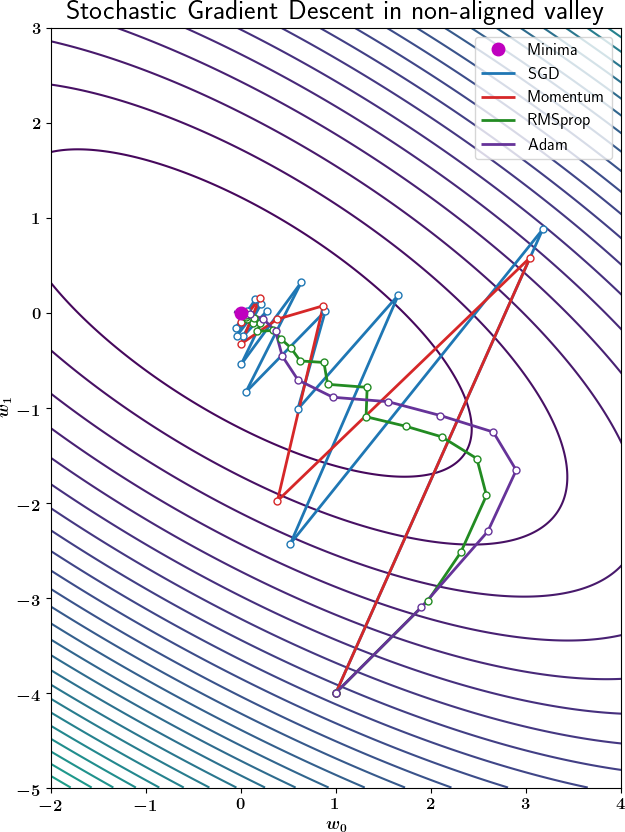
\includegraphics[width=100 mm]{images/nonaligned.png}
	\caption{Đường đi của các thuật toán trong rãnh hẹp có hướng không trùng với trọng số (b).}
	\label{fig:aligned-nonaligned}
\end{figure}

Trong trường hợp các hướng của rãnh hẹp không trùng với trục của trọng số (hình \ref{fig:aligned-nonaligned}b), thuật toán Adam không còn hiệu quả như khi trùng với trục trọng số. Mặc dù Adam vẫn cho biên độ dao động nhỏ hơn Momentum theo hướng có độ dốc cao nhưng độ lớn bước cập nhật trên hướng có độ dốc thấp đã không còn lớn như trường hợp rãnh hẹp trùng với trục trọng số. Tuy nhiên, nhờ sử dụng thêm quán tính mà Adam vẫn giữ được kích thước bước cập nhật lớn hơn RMSprop càng về sau của quá trình huấn luyện; đồng thời Adam điều chỉnh hướng đi tốt hơn và có thể triệu tiêu hiện tượng ``zig zag'' của RMSprop. Từ thí nghiệm cho thấy, vì Adam kết hợp sử dụng quán tính với tỉ lệ học thích ứng nên thuật toán vẫn có thể hoạt động tốt trong trường hợp rãnh hẹp không trùng với trục của trọng số. Điều này cho thấy Adam phù hợp với nhiều dạng địa hình khác nhau trong bề mặt lỗi.

\subsection{So sánh Adam với các thuật toán khác trong trường hợp bề mặt lỗi có dạng rãnh rất hẹp}
\label{exp:sparse-noisy}

Đặc trưng thưa là những đặc trưng mang giá trị 0 hoặc gần bằng 0 tại đa số các điểm dữ liệu; ngược lại, ta có đặc trưng đặc. Số lần các đặc trưng thưa được cập nhật là rất ít hoặc cập nhật với lượng rất nhỏ, từ đó kéo dài quá trình huấn luyện mạng nơ-ron nhiều tầng ẩn. Thêm nữa, đặc trưng thưa xuất hiện ở hầu hết các bài toán ứng dụng mạng nơ-ron sâu hiện nay nên đây là vấn đề cần được giải quyết.

Để quan sát cách các thuật toán tối ưu hoạt động với dữ liệu thưa, thí nghiệm sử dụng dữ liệu là $n$ cặp $(x,y)$, với $n = 1000$ được khởi tạo ngẫu nhiên. Sau đó, chọn $90\%$ trong số $n$ cặp và gán giá trị $x = 0$ với mục đích là khiến cho đặc trưng $x$ thưa. Sử dụng hàm mục tiêu có dạng $y = wx + b$, các thuật toán được sử dụng để tối ưu hàm chi phí $MSE = \frac{1}{n}\sum_{i=1}^n(y - wx - b)^2$. Kết quả độ lỗi sau 20 epoch với kích thước minibatch bằng 100 được thể hiện như trong hình \ref{fig:sparse}b và hình \ref{fig:sparse}a thể hiện đường đi của các thuật toán trên bề mặt lỗi. Vì đặc trưng có giá trị gần bằng 0 chiếm đa số nên hướng tương ứng của đặc trưng đó trên mặt phẳng lỗi là một vùng có độ cong thấp cho độ lỗi các hướng gần bằng nhau. Kết hợp với hướng $b$ ứng với đặc trưng đặc có độ cong cao, bề mặt lỗi trong trường hợp này hình thành một rãnh rất hẹp do sự khác nhau giữa hai hướng là rất lớn.

\begin{figure}[htp]
	\centering
	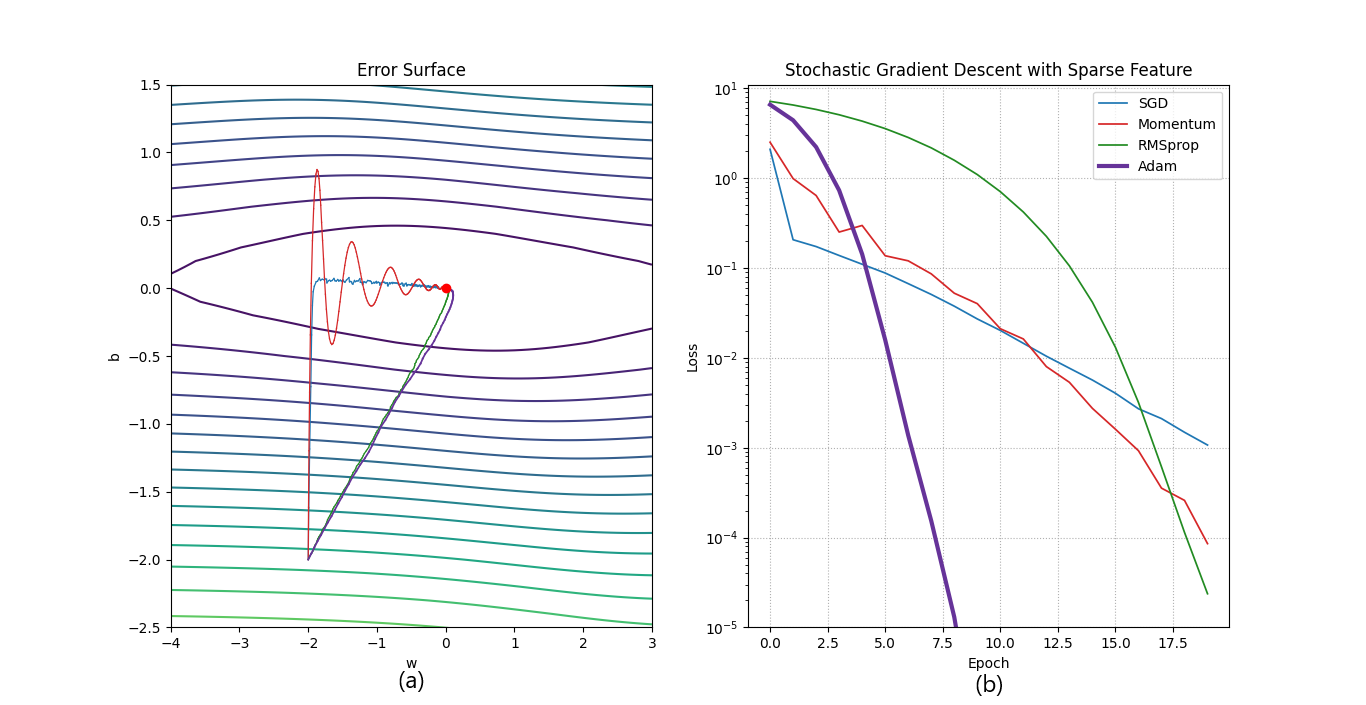
\includegraphics[width=130 mm]{images/sparse.png}
	\caption{Đường đi của các thuật toán trong bề mặt lỗi (a) và độ lỗi (b) của từng thuật toán trong trường hợp đặc trưng thưa.}
	\label{fig:sparse}
\end{figure}

Nhìn chung, thí nghiệm cho thấy thuật toán Adam là thuật toán hoạt động tốt nhất (cả về mặt độ lỗi lẫn thời gian huấn luyện) trong trường hợp bề mặt lỗi có dạng rãnh rất hẹp. Trong trường hợp này, một hệ số quán tính lớn cũng không đem lại nhiều lợi ích cho việc di chuyển theo hướng có độ cong thấp vì sẽ dẫn đến dao động cao trên hướng có độ cong cao và gần cực tiểu nên Momentum chỉ có thể di chuyển chậm theo hướng w. Vì cơ chế của tỉ lệ học thích ứng nên Adam và RMSprop có thể giảm bước cập nhật theo hướng có độ cong cao là b và tăng cường độ dài bước cập nhật trên hướng có độ cong thấp w hiệu quả hơn Momentum. Tuy nhiên, vì có khả năng tăng tốc bằng quán tính nên Adam cho thời gian huấn luyện chỉ bằng một nửa RMSprop để tới được điểm cực tiểu có độ lỗi nhỏ hơn các thuật toán khác.

\subsection{So sánh Adam với các thuật toán khác trong ngữ cảnh thực tế}

\subsubsection{Huấn luyện mô hình VGG16}
\label{exp:vgg16}

Chúng tôi thực hiện huấn luyện kiến trúc mạng tích chập nhiều tầng ẩn VGG16 của Karen Simonyan và Andrew Zisserman \cite{simonyan2014verydeep} trên tập dữ liệu ImageNet. Đây là một kiến trúc mạng nơ-ron nhiều tầng ẩn được sử dụng rộng rãi trong rất nhiều bài toán khác nhau do khả năng trích xuất đặc trưng rất mạnh. Kiến trúc mạng VGG16 cũng thường được sử dụng làm thước đo đánh giá độ hiệu quả của các thuật toán huấn luyện mạng nơ-ron nhiều tầng ẩn \cite{zhuang2020adabelief}\cite{schneider2018deepobs} do số lượng trọng số cũng như số lượng tầng ẩn rất lớn (khoảng 138 triệu trọng số và 16 tầng ẩn). Các thiết lập huấn luyện như kích thước minibatch, kích thước và quá trình tiền xử lý ảnh đầu vào được giữ nguyên như trong bài báo gốc của VGG16 \cite{simonyan2014verydeep}.

Với mỗi thuật toán tối ưu, chúng tôi cố gắng dò tìm bộ siêu tham số cho kết quả tốt nhất. Tuy nhiên, do việc huấn luyện mạng VGG16 với khoảng 138 triệu tham số trên một tập dữ liệu lớn như ImageNet rất tốn kém nên chúng tôi không thể dò tìm siêu tham số một cách chi tiết như các thí nghiệm khác. Một trường hợp đặc biệt là thuật toán SGD dường như không thể tối ưu cho kiến trúc mạng này khi độ lỗi luôn giữ ở mức cao bất kể siêu tham số mà chúng tôi thử nghiệm, vì vậy chúng tôi không bao gồm biểu đồ của SGD trong kết quả. Các siêu tham số được sử dụng trong thí nghiệm được trình bày trong bảng \ref{tab:vgg16-hparam}.

\begin{figure}[htp]
	\centering
	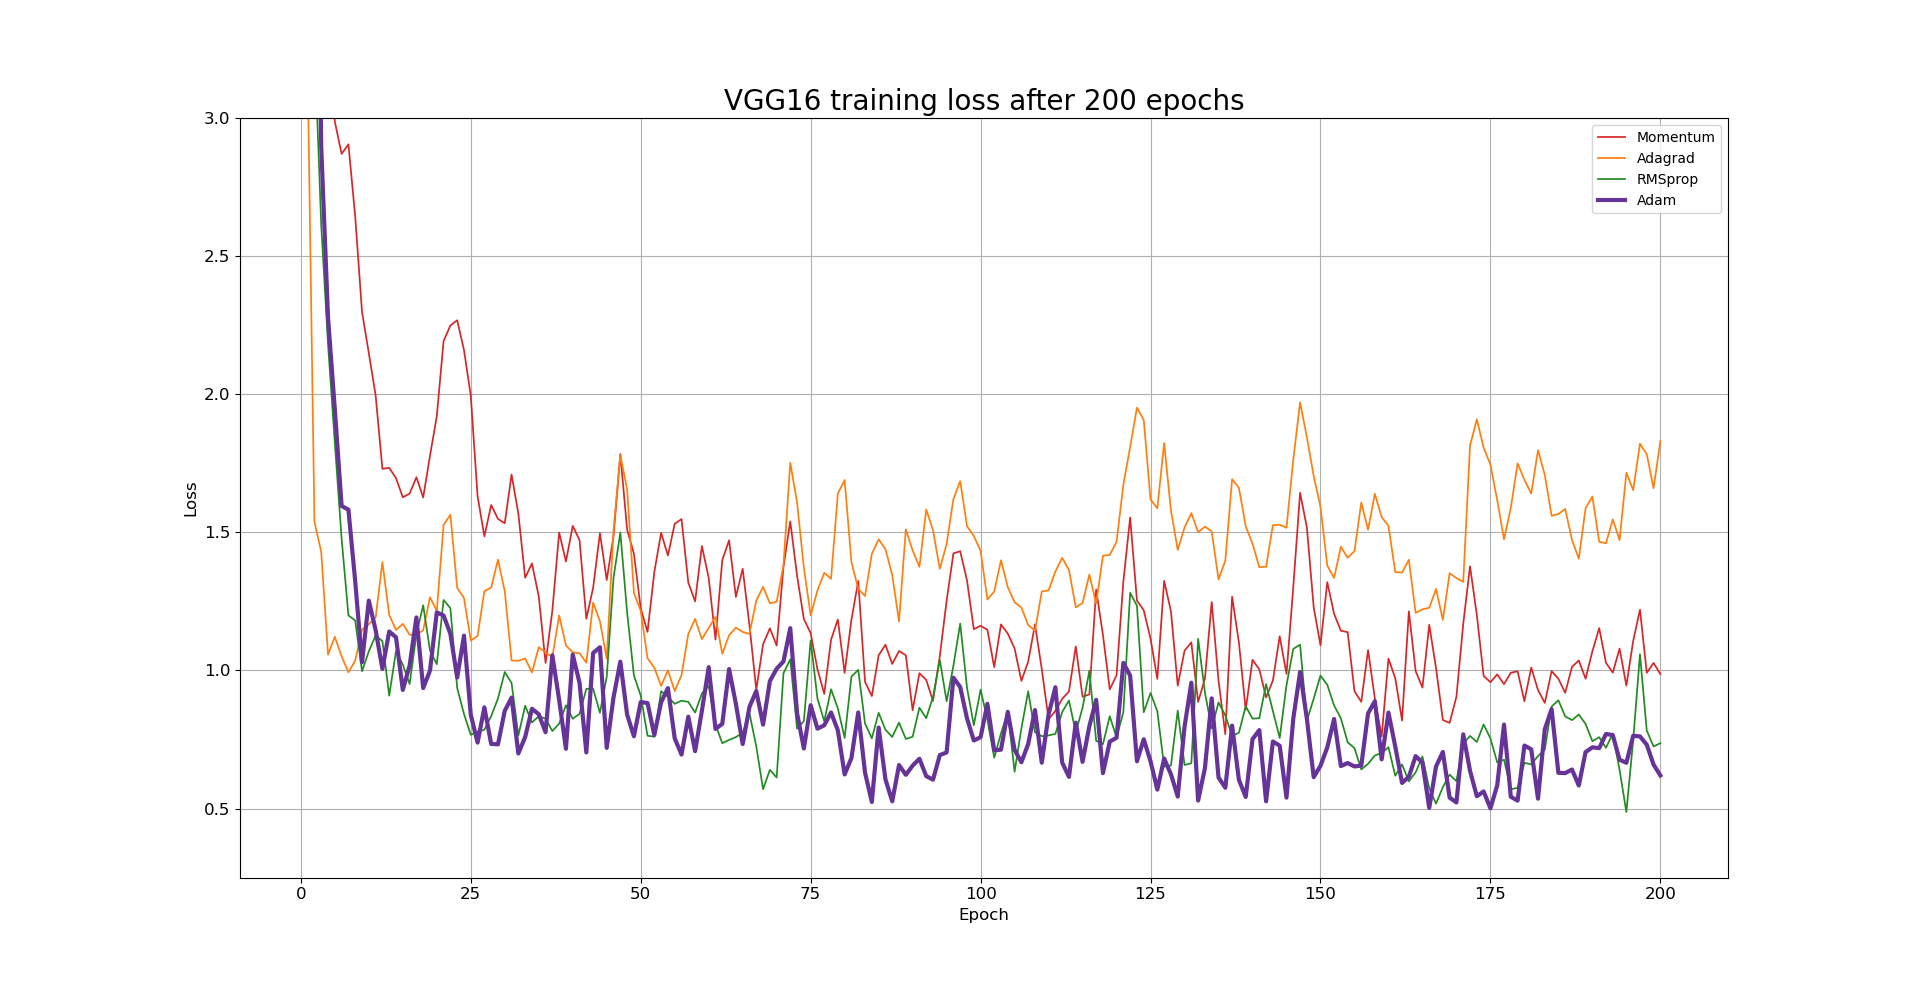
\includegraphics[width=140 mm]{images/vgg16.png}
	\caption{Đường đi của các thuật toán trong bề mặt lỗi (trái) và độ lỗi (phải) của từng thuật toán trong trường hợp đặc trưng thưa.}
	\label{fig:vgg16-loss}
\end{figure}

Quá trình huấn luyện mô hình VGG16 trên tập dữ liệu ImageNet (hình \ref{fig:vgg16-loss}) cho thấy Adam là thuật toán hiệu quả nhất trong số các thuật toán được thí nghiệm khi có độ lỗi giảm nhanh chóng và ổn định. Trái lại, Adagrad không những có độ dao động khá cao mà còn có xu hướng cho độ lỗi tăng trong những epoch cuối của quá trình huấn luyện, trở thành thuật toán có độ lỗi cao nhất. Thuật toán Momentum cho độ lỗi thấp thứ ba (sau RMSprop và Adam) nhưng sự chênh lệch độ lỗi giữa Momentum và Adam là rất lớn. Chỉ RMSprop là có độ lỗi gần với Adam nhất, nhưng RMSprop cũng có biên độ dao động lớn hơn.

\subsubsection{Huấn luyện mô hình ngôn ngữ}
\label{exp:lstm}

Chúng tôi sử dụng thiết lập giống trong bài báo của Zaremba và cộng sự \cite{zaremba2014recurrent} cho mô hình LSTM-medium. Sử dụng kiến trúc mạng RNN gồm 2 tầng Long short-term memory (LSTM), mỗi tầng có 650 nơ-ron với số bước unroll là 35. Chúng tôi khởi khởi tạo hai tầng ẩn này bằng giá trị 0 và sử dụng trạng thái ẩn cuối cùng của minibatch $t$ làm giá trị khởi tạo của trạng thái ẩn của minibatch t+1 với kích thước của một minibatch là 20.

Các giá trị trọng số trong mạng được khởi tạo theo phân phối đều trong khoảng [-0.05,0.05]. Với tỷ lệ dropout là 0.5 cho các liên kết không hồi quy, mô hình được huấn luyện trong 39 epoch với tỷ lệ học được tuning tốt nhất cho mỗi thuật toán tối ưu và được trình bày trong bảng \ref{tab:lstm-hparam}. Trong quá trình huấn luyện, sau epoch thứ 6 thì tỷ lệ học sẽ được nhân với $\frac{5}{6}$ sau mỗi epoch. Để hạn chế hiện tượng gradient bất ổn định, ta sử dụng ``gradient clipping'' - kĩ thuật giới hạn giá trị tuyệt đối của gradient - với giá trị giới hạn là 5.

\begin{figure}[htp]
	\centering
	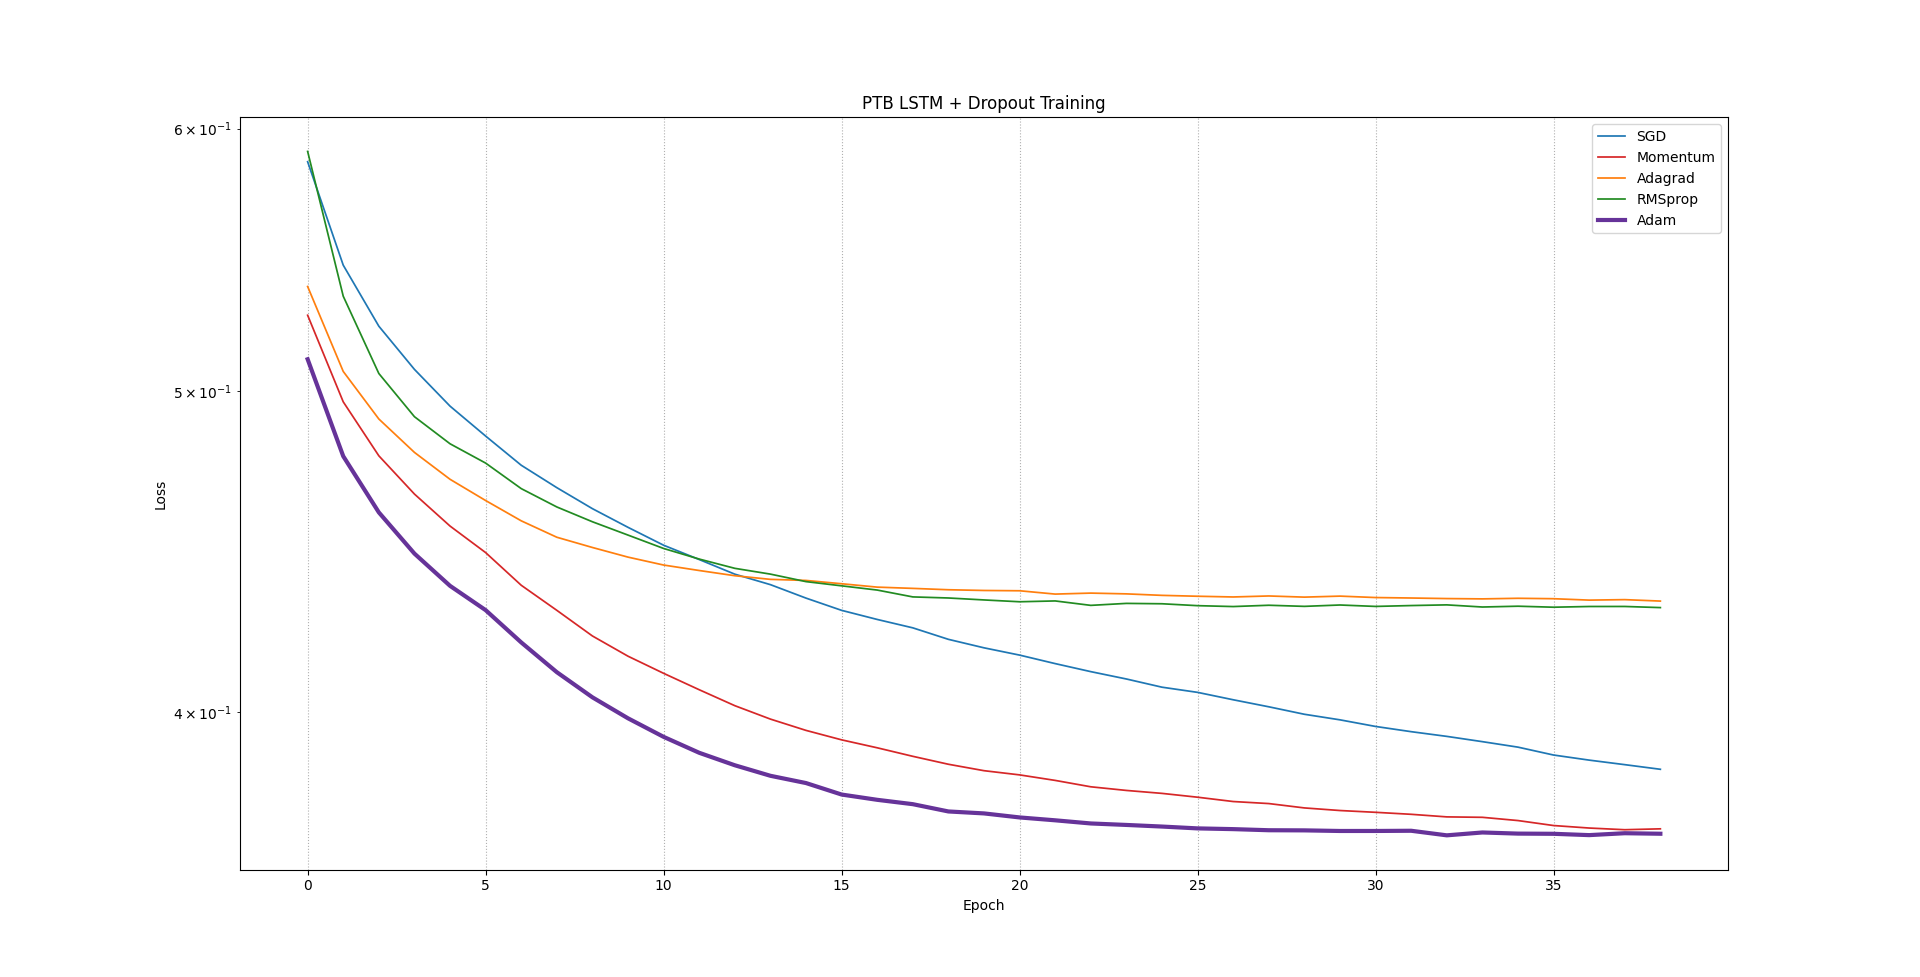
\includegraphics[width=140 mm]{images/ptb.png}
	\caption{Độ lỗi huấn luyện mô hình ngôn ngữ trên tập Penn TreeBank có sử dụng gradient clipping..}
	\label{fig:ptb}
\end{figure}

Hình \ref{fig:ptb} cho ta kết quả chạy của mô hình LSTM trên tập Penn Treebank trong 39 epoch. Nhìn chung Adam vẫn có độ lỗi nhỏ nhất và thời gian tiêu tốn ít nhất để tìm được đến độ lỗi này. Ta thấy được rằng Adam cho độ lỗi nhỏ nhất ngay từ những epoch đầu tiên, theo ngay sau đó là Momentum. Trong khi Adam vẫn còn tiếp tục di chuyển về vùng có độ lỗi nhỏ hơn, RMSprop và Adagrad đã bị chững lại tại điểm có độ lỗi khá cao. Thuật toán SGD vẫn tiếp tục đi xuống mặc dù tốc độ di chuyển chậm hơn Adam và Momentum. Có thể thấy rằng trong trường hợp trên, hai thuật toán SGD và Momentum cho độ lỗi thấp rất gần với Adam, trong đó Momentum đuổi kịp Adam tại những epoch cuối còn SGD mặc dù di chuyển chậm nhưng có xu hướng tiến gần hơn tới Adam và có thể đạt cùng độ lỗi với số lượng epoch lớn hơn. Giả thiết cho rằng việc giới hạn trung bình của gradient đã khiến cho trường hợp giá trị gradient rất khác nhau xảy ra rất ít, những vùng này là thế mạnh của các thuật toán Momentum và SGD giải thích lý do tại sao hai thuật toán này có thể bắt kịp với Adam.

\begin{figure}[htp]
	\centering
	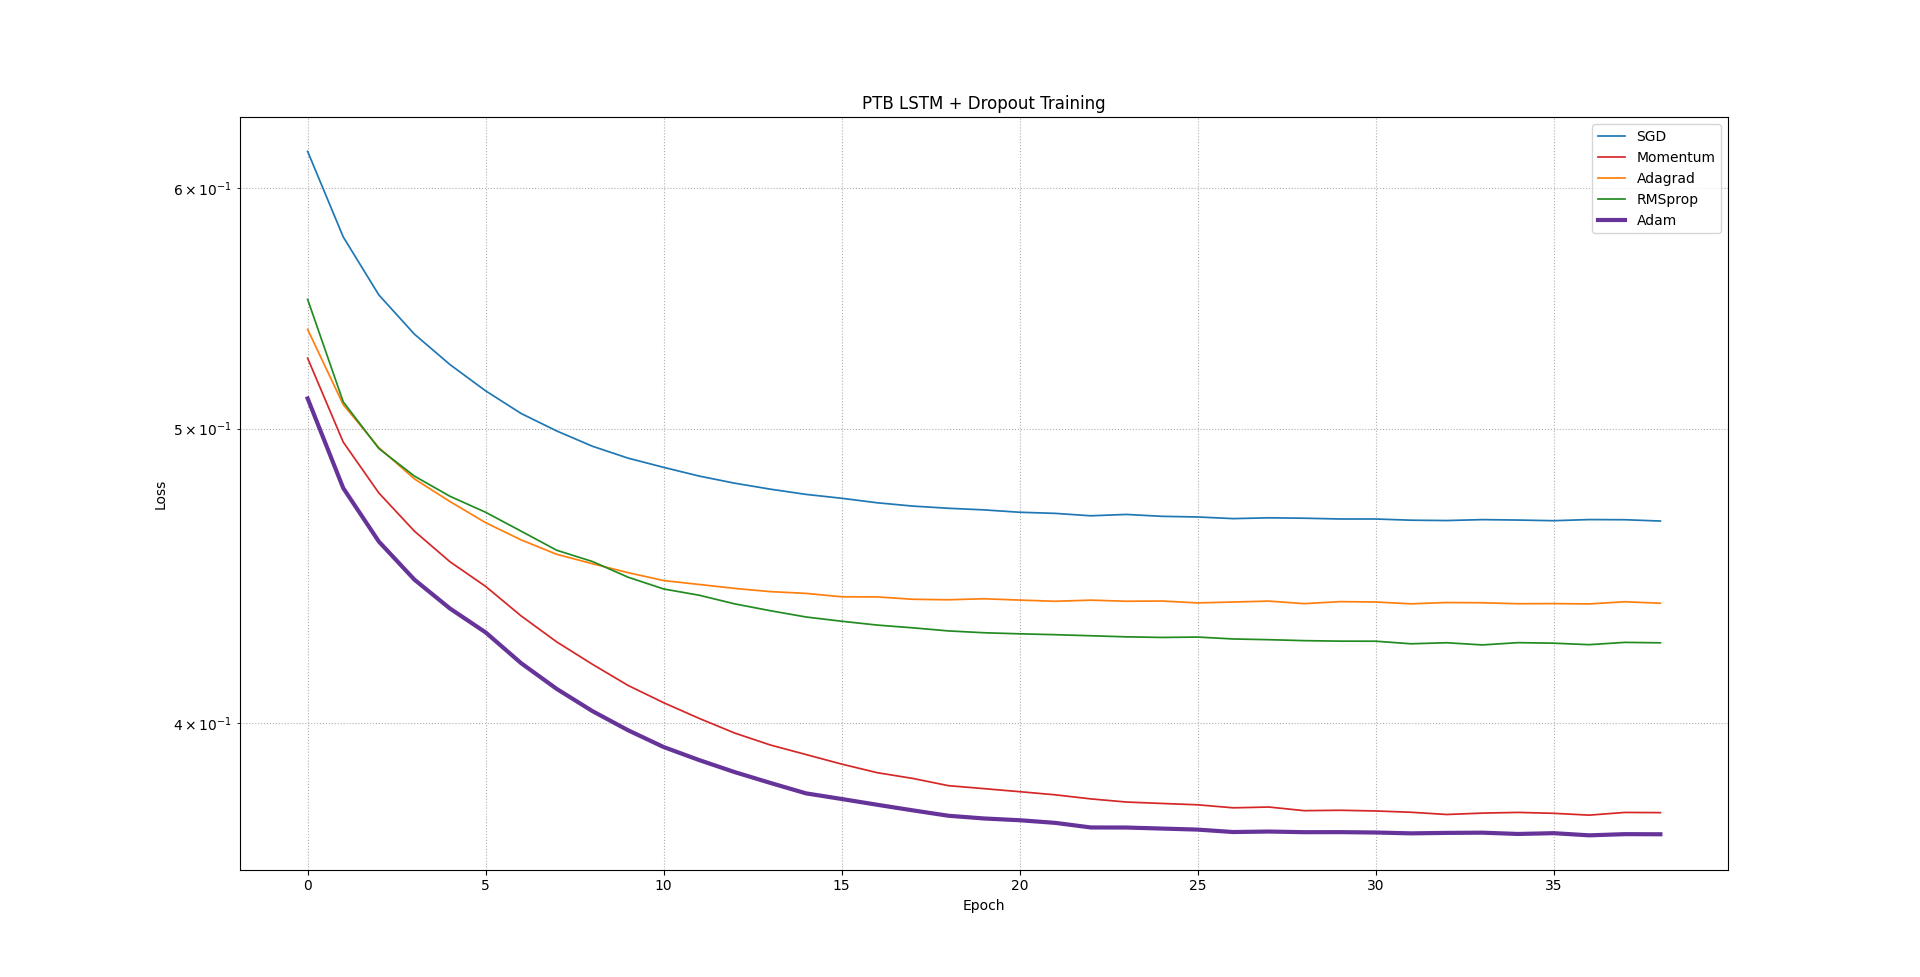
\includegraphics[width=140 mm]{images/ptb2.png}
	\caption{Độ lỗi huấn luyện mô hình ngôn ngữ trên tập dữ liệu Penn TreeBank không sử dụng gradient clipping.}
	\label{fig:ptb2}
\end{figure}

Hình \ref{fig:ptb2} là kết quả chạy của mô hình khi không giới hạn độ lớn của trung bình gradient. Nhìn tổng thể, ta có thể thấy Adam vẫn là thuật toán cho độ lỗi thấp nhất trong các thuật toán. Nếu ở trường hợp trước, SGD có thể gần như bắt kịp Adam thì ở đây SGD chững lại khá sớm và cho độ lỗi cao nhất trong năm thuật toán. Đây có thể là minh chứng cho giả thiết được đặt ra ở trường hợp trên. Ở đây bề mặt lỗi gồm nhiều vùng rãnh hẹp, các vùng này khiến SGD có độ lỗi giảm rất chậm tạo cảm giác thuật toán bị chững lại. Mặc dù Adagrad và RMSprop đã có sự cải thiện về mặt độ lỗi nhưng vẫn không thể tiến gần đến độ lỗi của Adam trước khi bị đi ngang. Nếu ở thí nghiệm trước, thuật toán Momentum gần như đuổi kịp Adam thì ở thí nghiệm này đã có một sự cách biệt giữa độ lỗi của hai thuật toán (từ 0,002 tăng lên 0,009). Thuật toán Adam vẫn cho độ lỗi trong tập huấn luyện là nhỏ nhất trong các thuật toán.

Các giá trị độ lỗi và thời gian chạy tương ứng với từng thuật toán được trình bày trong bảng \ref{tab:lstm-results}. Độ lỗi được thể hiện trong bảng bao gồm độ lỗi thấp nhất và cao nhất trong quá trình huấn luyện trên cả hai tập huấn luyện và tập kiểm thử.

\begin{table}
	\begin{adjustbox}{width=1\textwidth}
	\small
	\begin{tabular}{|l|>{\raggedright\arraybackslash}m{0.17\textwidth}|>{\raggedright\arraybackslash}m{0.14\textwidth}|>{\raggedright\arraybackslash}m{0.14\textwidth}|>{\raggedright\arraybackslash}m{0.125\textwidth}|>{\raggedright\arraybackslash}m{0.125\textwidth}|}
		\hline
		\textbf{Thuật toán} & \textbf{Thời gian thực hiện (giây)} & \textbf{Độ~lỗi huấn~luyện} & \textbf{Độ Perp. huấn~luyện} & \textbf{Độ~lỗi kiểm~thử} & \textbf{Độ Perp. kiểm~thử} \\
		\hline
		\multirow{2}{*}{SGD} & \textbf{21.78}        & 0.47 & 1.59 & 4.90 & 134.27 \\
							 & \textbf{$\pm$0.00023} & 0.62 & 1.85 & 6.39 & 593.27 \\
		\hline
		\multirow{2}{*}{Momentum} & \multirow{2}{*}{22.61$\pm$0.00025} & 0.37 & 1.45 & \textbf{4.40} & \textbf{81.82} \\
								  &                                    & 0.53 & 1.70 & \textbf{5.41} & \textbf{223.34} \\
		\hline
		\multirow{2}{*}{Adagrad} & \multirow{2}{*}{23.27$\pm$0.0054} & 0.44 & 1.54 & 4.71 & 110.94 \\
								 &                                   & 0.54 & 1.72 & 5.52 & 250.73 \\
		\hline
		\multirow{2}{*}{RMSprop} & \multirow{2}{*}{23.60$\pm$0.013} & 0.43 & 1.54 & 4.71 & 111.44 \\
								 &                                  & 0.59 & 1.80 & 6.00 & 402.50 \\
		\hline
		\multirow{2}{*}{Adam} & \multirow{2}{*}{26.21$\pm$0.46} & \textbf{0.37} & \textbf{1.44} & 4.47 & 87.78 \\
							  &                                 & \textbf{0.51} & \textbf{1.67} & 5.20 & 180.62 \\
		\hline
	\end{tabular}
	\end{adjustbox}
\caption{\label{tab:lstm-results}Kết quả và thời gian thực hiện một epoch của các thuật toán trong thí nghiệm Mô hình ngôn ngữ.}
\end{table}

Thông qua bảng dữ liệu \ref{tab:lstm-results}, ta thấy hiện tượng được Wilson và cộng sự đề cập trong bài báo \cite{wilson2017marginal}: mặc dù Adam cho độ lỗi nhỏ hơn Momentum trong tập huấn luyện nhưng lại cho kết quả độ lỗi ngoài tập huấn luyện cao hơn. Một số bài báo gần đây cố gắng đưa ra lời giải thích cho trường hợp thông qua lý thuyết về cực tiểu bằng phẳng (flat minima) thường nằm ở các vùng bằng phẳng hay tại đáy của các rãnh hẹp, ngược lại ta có cực tiểu nhọn (sharp minima). Dựa trên quan điểm các vùng cực tiểu bằng phẳng tổng quát hoá tốt hơn, Pan Zhou và cộng sự cho rằng lý do Adam có độ lỗi ngoài tập huấn luyện cao hơn SGD là do Adam dễ dàng hội tụ tại các vùng cực tiểu nhọn trong khi SGD lại có thể thoát khỏi vùng cực tiểu này để đến vùng cực tiểu bằng phẳng hơn \cite{zhou2020towards}. Tuy nhiên, vẫn có bài báo có quan điểm ngược lại, cho rằng: cực tiểu nhọn cho độ lỗi ngoài tập huấn luyện tốt hơn cực tiểu bằng \cite{li2018visualizing} nên đây vẫn chưa thể coi là lời giải thích chính thức cho hiện tượng này.